\documentclass[tikz,border=8pt]{standalone}
\usepackage{pgfplots}
\usepgfplotslibrary{groupplots}
\pgfplotsset{compat=1.18}
\begin{document}
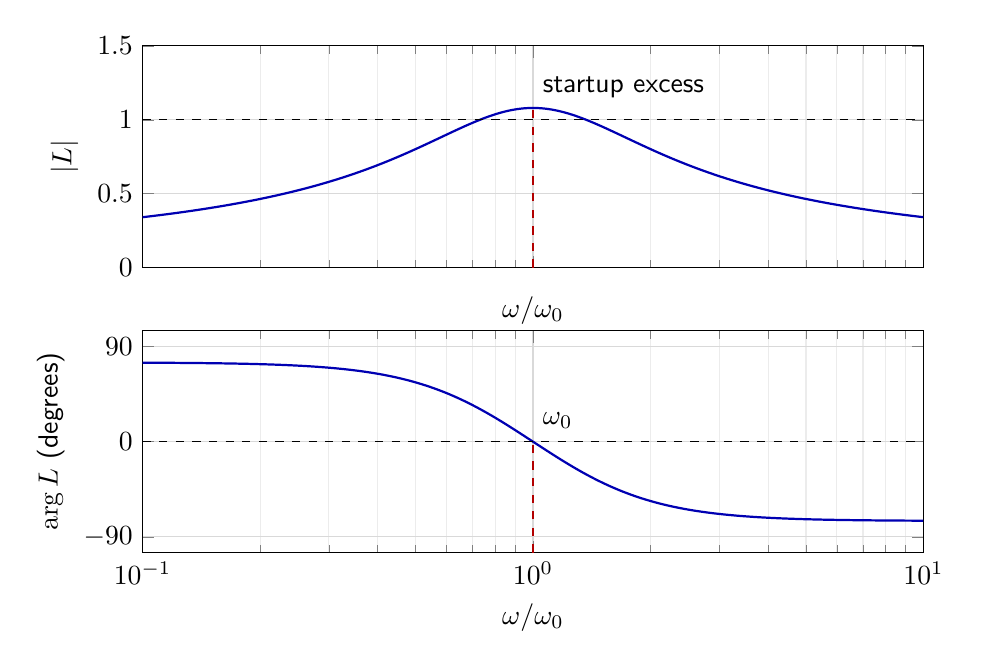
\begin{tikzpicture}[font=\sffamily]
\begin{groupplot}[group style={group size=1 by 2,vertical sep=8mm},width=11.5cm,height=4.4cm,xmode=log,xmin=.1,xmax=10,grid=both,minor grid style={gray!15},major grid style={gray!30},xlabel={$\omega/\omega_0$}]
\nextgroupplot[ylabel={$|L|$},ymin=0,ymax=1.5,xticklabels=\empty]
\addplot[blue!70!black,thick,domain=.1:10,samples=300] {1.08/sqrt(1+9*(ln(x)/ln(10))^2)};
\addplot[black,dashed] coordinates {(.1,1) (10,1)};
\draw[red!70!black,dashed] (axis cs:1,0)--(axis cs:1,1.08);
\node[above right] at (axis cs:1,1.08) {startup excess};
\nextgroupplot[ylabel={$\arg L$ (degrees)},ymin=-105,ymax=105,ytick={-90,0,90}]
\addplot[blue!70!black,thick,domain=.1:10,samples=300] {-75*tanh(1.4*ln(x))};
\addplot[black,dashed] coordinates {(.1,0) (10,0)};
\draw[red!70!black,dashed] (axis cs:1,-105)--(axis cs:1,0);
\node[above right] at (axis cs:1,3) {$\omega_0$};
\end{groupplot}
\end{tikzpicture}
\end{document}
